\documentclass{article}
\usepackage[paperwidth=7.35in,paperheight=5.20in,margin=0in]{geometry}
\usepackage{amsmath}
\usepackage{amssymb}
\usepackage{tikz}
\usetikzlibrary{arrows.meta,calc}
\pagestyle{empty}

% Editable probability-density parameters.
% This is deliberately different from the loss landscape extrema.
% Centers c_k=(u_k,v_k), weights w_k sum to 1, and sigma values set cluster spread.
\newcommand{\COneU}{-1.75}
\newcommand{\COneV}{0.15}
\newcommand{\COneW}{0.22}
\newcommand{\COneSu}{0.50}
\newcommand{\COneSv}{0.46}
\newcommand{\CTwoU}{-0.70}
\newcommand{\CTwoV}{-1.55}
\newcommand{\CTwoW}{0.19}
\newcommand{\CTwoSu}{0.58}
\newcommand{\CTwoSv}{0.44}
\newcommand{\CThreeU}{0.75}
\newcommand{\CThreeV}{1.45}
\newcommand{\CThreeW}{0.21}
\newcommand{\CThreeSu}{0.56}
\newcommand{\CThreeSv}{0.52}
\newcommand{\CFourU}{1.70}
\newcommand{\CFourV}{-0.55}
\newcommand{\CFourW}{0.18}
\newcommand{\CFourSu}{0.48}
\newcommand{\CFourSv}{0.60}
\newcommand{\CFiveU}{-0.10}
\newcommand{\CFiveV}{0.65}
\newcommand{\CFiveW}{0.20}
\newcommand{\CFiveSu}{0.72}
\newcommand{\CFiveSv}{0.50}

\newcommand{\densityheight}[2]{%
  \COneW*(1/(6.2831853*\COneSu*\COneSv))*exp(-0.5*(((#1)-(\COneU))/\COneSu)^2 -0.5*(((#2)-(\COneV))/\COneSv)^2)
  + \CTwoW*(1/(6.2831853*\CTwoSu*\CTwoSv))*exp(-0.5*(((#1)-(\CTwoU))/\CTwoSu)^2 -0.5*(((#2)-(\CTwoV))/\CTwoSv)^2)
  + \CThreeW*(1/(6.2831853*\CThreeSu*\CThreeSv))*exp(-0.5*(((#1)-(\CThreeU))/\CThreeSu)^2 -0.5*(((#2)-(\CThreeV))/\CThreeSv)^2)
  + \CFourW*(1/(6.2831853*\CFourSu*\CFourSv))*exp(-0.5*(((#1)-(\CFourU))/\CFourSu)^2 -0.5*(((#2)-(\CFourV))/\CFourSv)^2)
  + \CFiveW*(1/(6.2831853*\CFiveSu*\CFiveSv))*exp(-0.5*(((#1)-(\CFiveU))/\CFiveSu)^2 -0.5*(((#2)-(\CFiveV))/\CFiveSv)^2)%
}
\newcommand{\projectpoint}[3]{%
  ({94 + 16*(#1) - 16*(#2)},
   {42 - 6*(#1) - 6*(#2) + 115*(#3)})%
}

\begin{document}
\noindent
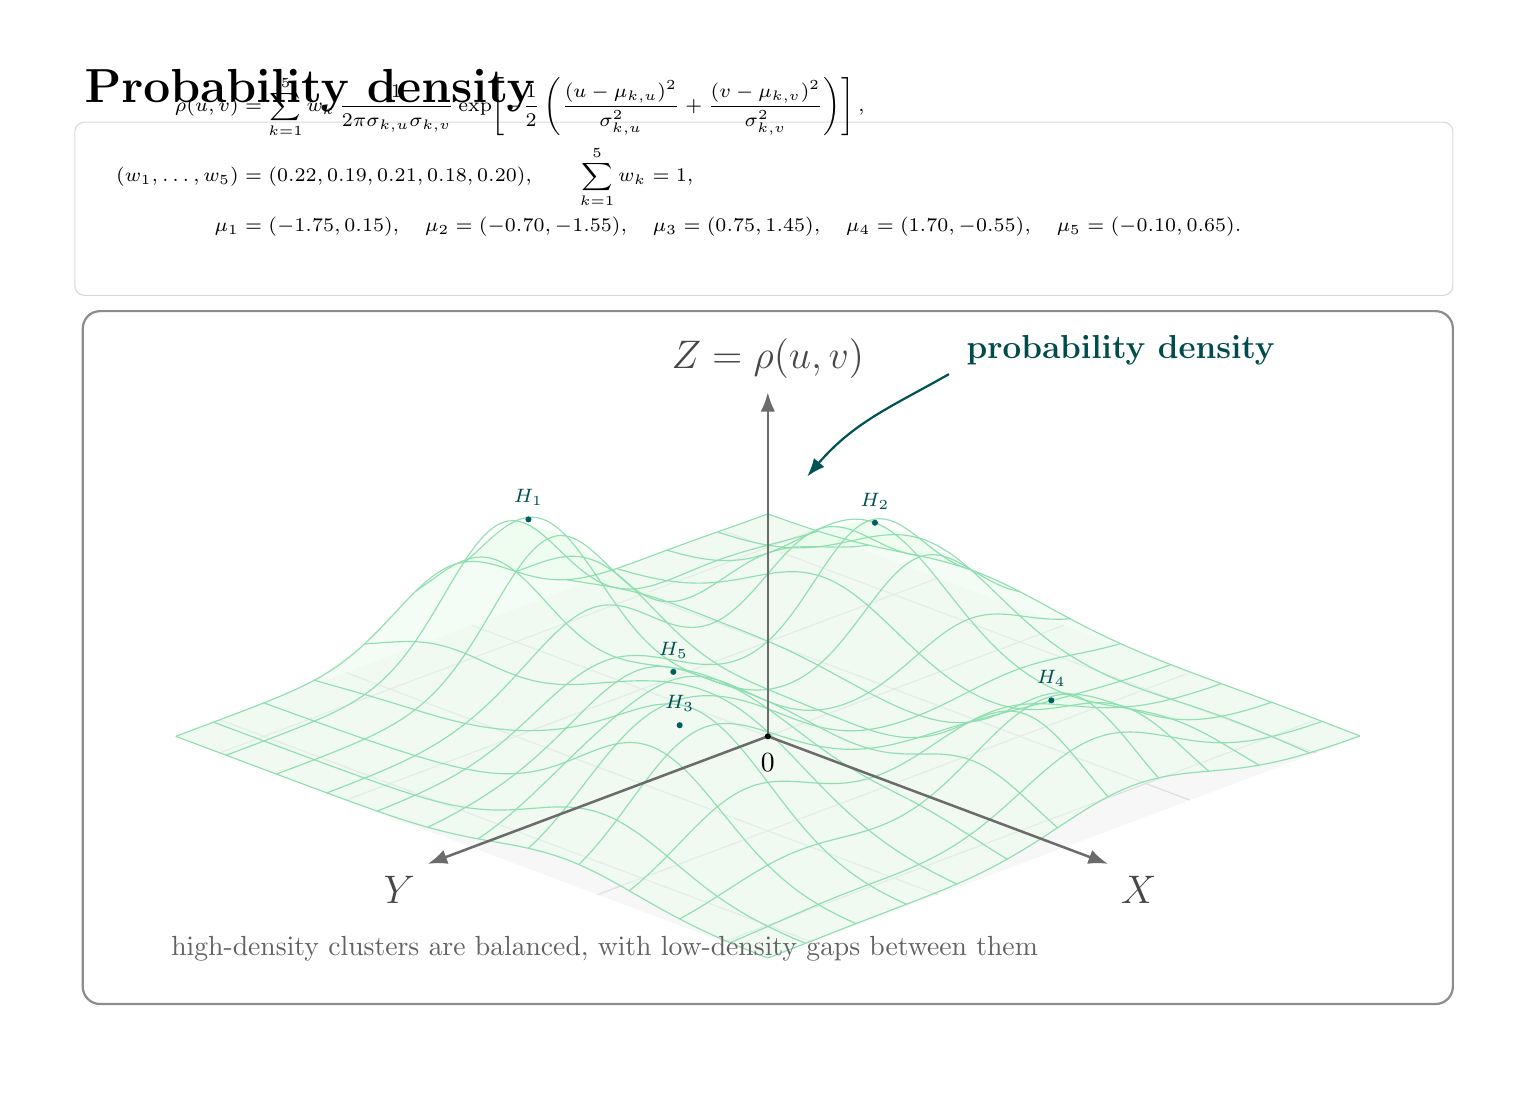
\begin{tikzpicture}[
  x=1mm,y=1mm,
  >=Latex,
  font=\sffamily,
  panel/.style={draw=black!45, rounded corners=2.2mm, line width=0.8pt, fill=white},
  axis/.style={->, draw=black!58, line width=0.9pt},
  floorgrid/.style={draw=black!13, line width=0.4pt},
  meshline/.style={draw=teal!58!green!45!white, line width=0.42pt, opacity=0.95},
  surfacepatch/.style={fill=teal!20!green!8!white, fill opacity=0.50, draw=none},
  formula/.style={font=\scriptsize, align=left, anchor=west},
  axislabel/.style={font=\Large, text=black!72},
  densitylabel/.style={font=\large\bfseries, text=teal!60!black}
]
\path[use as bounding box] (0,0) rectangle (186,132);

% Header
\node[font=\LARGE\bfseries, anchor=west] at (6,124)
  {Probability density};

% Formula box
\fill[white, opacity=0.94] (6,98) rectangle (181,120);
\draw[black!15, rounded corners=1.2mm] (6,98) rectangle (181,120);
\node[formula] at (10,115.6)
  {$\displaystyle\begin{aligned}
    \rho(u,v)&=\sum_{k=1}^{5}w_k\,
      \frac{1}{2\pi\sigma_{k,u}\sigma_{k,v}}
      \exp\!\left[-\frac12\left(
      \frac{(u-\mu_{k,u})^2}{\sigma_{k,u}^2}
      +\frac{(v-\mu_{k,v})^2}{\sigma_{k,v}^2}\right)\right],\\[-0.4mm]
    (w_1,\ldots,w_5)&=(0.22,0.19,0.21,0.18,0.20),\qquad
      \sum_{k=1}^{5}w_k=1,\\[-0.4mm]
    \mu_1&=(-1.75,0.15),\quad
    \mu_2=(-0.70,-1.55),\quad
    \mu_3=(0.75,1.45),\quad
    \mu_4=(1.70,-0.55),\quad
    \mu_5=(-0.10,0.65).
  \end{aligned}$};

% Main panel
\draw[panel] (7,8) rectangle (181,96);

\begin{scope}
  \clip (8,9) rectangle (180,95);

  % Faint XY reference plane below the density surface.
  \fill[black!4, opacity=0.80]
    \projectpoint{-2.35}{-2.35}{0} --
    \projectpoint{ 2.35}{-2.35}{0} --
    \projectpoint{ 2.35}{ 2.35}{0} --
    \projectpoint{-2.35}{ 2.35}{0} -- cycle;
  \foreach \t in {-2,-1,0,1,2} {
    \draw[floorgrid] \projectpoint{-2.35}{\t}{0} -- \projectpoint{2.35}{\t}{0};
    \draw[floorgrid] \projectpoint{\t}{-2.35}{0} -- \projectpoint{\t}{2.35}{0};
  }

  % Transparent filled density surface patches.
  \foreach \ya/\yb in {-2.35/-1.95,-1.95/-1.55,-1.55/-1.15,-1.15/-0.75,-0.75/-0.35,-0.35/0.05,0.05/0.45,0.45/0.85,0.85/1.25,1.25/1.65,1.65/2.05,2.05/2.35} {
    \foreach \xa/\xb in {-2.35/-1.95,-1.95/-1.55,-1.55/-1.15,-1.15/-0.75,-0.75/-0.35,-0.35/0.05,0.05/0.45,0.45/0.85,0.85/1.25,1.25/1.65,1.65/2.05,2.05/2.35} {
      \path[surfacepatch]
        \projectpoint{\xa}{\ya}{\densityheight{\xa}{\ya}} --
        \projectpoint{\xb}{\ya}{\densityheight{\xb}{\ya}} --
        \projectpoint{\xb}{\yb}{\densityheight{\xb}{\yb}} --
        \projectpoint{\xa}{\yb}{\densityheight{\xa}{\yb}} -- cycle;
    }
  }

  % Smooth mesh lines on the density surface.
  \foreach \yy in {-2.35,-1.95,-1.55,-1.15,-0.75,-0.35,0.05,0.45,0.85,1.25,1.65,2.05,2.35} {
    \draw[meshline]
      plot[domain=-2.35:2.35, samples=58, variable=\x, smooth]
      ({94 + 16*\x - 16*(\yy)},
       {42 - 6*\x - 6*(\yy) + 115*(\densityheight{\x}{\yy})});
  }
  \foreach \xx in {-2.35,-1.95,-1.55,-1.15,-0.75,-0.35,0.05,0.45,0.85,1.25,1.65,2.05,2.35} {
    \draw[meshline]
      plot[domain=-2.35:2.35, samples=58, variable=\y, smooth]
      ({94 + 16*(\xx) - 16*\y},
       {42 - 6*(\xx) - 6*\y + 115*(\densityheight{\xx}{\y})});
  }

  % Mark high-density cluster centers. They do not coincide with loss extrema.
  \foreach \u/\v/\lab in {
    \COneU/\COneV/H_1,
    \CTwoU/\CTwoV/H_2,
    \CThreeU/\CThreeV/H_3,
    \CFourU/\CFourV/H_4,
    \CFiveU/\CFiveV/H_5
  } {
    \fill[teal!75!black] \projectpoint{\u}{\v}{\densityheight{\u}{\v}}
      circle[radius=1.1pt];
    \node[font=\scriptsize\bfseries, text=teal!62!black, above=0.5mm]
      at \projectpoint{\u}{\v}{\densityheight{\u}{\v}} {$\lab$};
  }
\end{scope}

% Coordinate axes facing the viewer: same XY slice as the loss landscape.
\coordinate (O) at (94,42);
\draw[axis] (O) -- \projectpoint{2.70}{0}{0}
  node[axislabel, below right=0.3mm] {$X$};
\draw[axis] (O) -- \projectpoint{0}{2.70}{0}
  node[axislabel, below left=0.3mm] {$Y$};
\draw[axis] (O) -- \projectpoint{0}{0}{0.38}
  node[axislabel, above=0.4mm] {$Z=\rho(u,v)$};
\fill[black] (O) circle[radius=1.1pt] node[below=1mm, font=\normalsize] {$0$};

\node[densitylabel, anchor=west] at (118,91) {probability density};
\draw[->, draw=teal!65!black, line width=0.8pt]
  (117,88) .. controls (110,84) and (105,82) .. (99,75);
\node[font=\normalsize, text=black!62, anchor=west] at (17,15)
  {high-density clusters are balanced, with low-density gaps between them};

\end{tikzpicture}
\end{document}
